In this chapter I will provide the reader with the basic understanding of the concept of neural networks and the surrounding field. We will look at the general topic of machine learning, explain the place of neural networks as machine learning algorithms, explore different types of neural network architectures and so on. When it comes to OOP, it is very important to understand the entity that we are trying to represent in our code on a deep level. We must know what exactly is, and what isn’t a neural network, what are the different types of networks, how are they different. What is the relation between a neural network and a neuron? Finally, when it comes to weights, are they properties of a neuron, or of a whole network? If it’s neuron, then which neuron should store these weights, the one that receives the signal, or the one that emits it?

\section{What is machine learning?}
In recent years Machine Learning became one of the most promising and rapidly developing fields in Computer Science. It tackles the problems that classical programming and sometimes also humans can't handle. In this section I will give the short introduction to the field of Machine Learning.

In his book \textit{Information Theory, Inference, and Learning Algorithms} \cite{MacKay-2003} David MacKay writes:
  \begin{quote}
    Machine learning allows us to tackle tasks that are too difficult to solve with fixed programs written and designed by human beings. From a scientific and philosophical point of view, machine learning is interesting because developing our understanding of machine learning entails developing our understanding of the principles that underlie intelligence.
  \end{quote}
  
  \paragraph{Definition}
  % TODO: Cite something here
  The intuitive definition of machine learning was given by Arthur Samuel in 1959:
  
  \begin{quote}
    Machine Learning is a field of study that gives computers the ability to learn without being explicitly programmed.
  \end{quote}
  
  This definition is nice and easy to understand. Though, to work with machine learning as a scientific field (indeed, it is a field of computer science, strongly related to some mathematical fields, such as computational statistics and mathematical optimization), we need a more formal definition. One can be found in Tom Mitchell's book \textit{Machine Learning} (1997) \cite{Mitchell-1997}. This definition is widely known and often reffered to as a well-posed learning problem:
  
  \begin{quote}
  A computer program is said to learn from experience $ E $ with respect to some class of tasks $ T $ and performance measure $ P $, if its performance at tasks in $ T $, as measured by $ P $, improves with experience $ E $.
  \end{quote}
  
  \paragraph{Machine learning problems}
  By the way we measure performance $ P $ on task $ T $ machine learning tasks can be divided into three main classes:
  
  \begin{itemize}
    \item \textbf{Supervised Learning} - the agent receives the set of examples with labels ("right answers") to learn from
    \item \textbf{Unsupervised Learning} - no explicit feedback is provided. The agent should learn patterns in an unlabeled dataset
    \item \textbf{Reinforcement Learning} - the agent receives series of reinforcements - rewards or punishments (for example, winning or loosing the chess game)
  \end{itemize}
  
  Here are the formal definitions for the problems of supervised and unsupervised machine learning\footnote{Formal definitions of supervised and unsupervissed learning problems are inspired by \cite{Russell-Norvig-2010} and \cite{Raina-et-al-2009} respectively}.
  
  \paragraph{Task of supervised learning}
  Given a training set of $ m $ example input-output pairs
  \[ (x^{(1)}, y^{(1)}), (x^{(2)}, y^{(2)}), ..., (x^{(m)}, y^{(m)}) \]
  where each $ y^{(j)} $ is generated by an unknown function $ y^{(j)} = f(x^{(j)}) $
  
  \textbf{Goal:} discover the function $ h $ that approximates function $ f $.
  
  \paragraph{Task of unsupervised learning}
  Given a large unlabeled dataset of $ m $ input examples
  \[ x^{(1)}, x^{(2)}, ..., x^{(m)} \]
  where each $ x^{(i)} \in \mathbb{R}^{n} $.
  
  \textbf{Goal:} learn a model for the inputs and then apply it to a specific machine learning task.
  
  %TODO: Add task of reinforcement learning
  %TODO: Write about classification and regression


\section{Neural networks}
An artificial neural networks is one of the most developed and widely used algorithms of machine learning.
It is the mathematical model of brain's activity that is able to tackle both problems of classification and regression. Neural network can function as a model of supervised, unsupervised or reinforcement learning. 
  
\paragraph{Definition}
Simon Haykin \cite{Haykin-2005} offers the following definition:
\begin{quote}
  A neural network is a massively parallel distributed processor made up of simple processing units, which has a natural propensity for storing experiential knowledge and making it available for use. It resembles brain in two respects:
  \begin{enumerate}
    \item Knowledge is aquired by network from its environment through a learning process.
    \item Interneuron connection strengths, known as synaptic weights, are used to store the acquired knowledge.
  \end{enumerate}
\end{quote}

Since their invention in 50-s neural networks have been used to model human brain and approach the goal of creating human-like artificial intelligence. Nowadays it is more common to think of neural networks as of the statistical models that perform well on some extremely complicated tasks. For example, Hastie et. al. \cite{Hastie-et-al-2013} view neural networks as nonlinear statistical models, the two-stage regression or classification models. David MacKay \cite{MacKay-2003} sees them as parallel distributed computational systems consisting of many interacting simple elements. And Goodfellow et. al. (MIT) \cite{Goodfellow-et-al-2016} write the following

\begin{quote}
  Modern neural network research is guided by many mathematical and engineering disciplines, and the goal of neural networks is not to perfectly model the brain. It is best to think of feedforward networks as function approximation machines that are designed to achieve statistical generalization, occasionally drawing some insights from what we know about the brain, rather than as models of brain function.
\end{quote}


\section{Model of a neuron}
A biological neural network (brain) consists of cells called neurons. Human brain is composed of about 10 billion neurons, each connected to about 10,000 other neurons. The same applies to artificial neural network - they consists of many artificial neurons - mathematical models of biological ones. I will start this section by describing the structure of a biological neuron. Then I will provide a formal description of an artificial neuron as a mathematical model.

\paragraph{Biological neurons} According to the medical definition, provided by Merriam-Webster dictionary\footnote{http://www.merriam-webster.com/dictionary/neuron},
\begin{quote}
  Neuron is a cell that carries messages between the brain and other parts of the body and that is the basic unit of the nervous system.
\end{quote}

Figure \ref{fig:bioneuron} shows the simplified schematic of a biological neuron. Each neuron consists of a cell body, or soma, that contains a cell nucleus. Branching out from the cell body are a number of fibers called dendrites and a single long fiber called the axon. The axon stretches out for a long distance, much longer than the scale in this diagram indicates. Typically, an axon is 1 cm long (100 times the diameter of the cell body), but can reach up to 1 meter. A neuron makes connections with 10 to 100,000 other neurons at junctions called synapses. Signals are propagated from neuron to neuron by a complicated electrochemical reaction. The signals control brain activity in the short term and also enable long-term changes in the connectivity of neurons. These mechanisms are thought to form the basis fur learning in the brain.
Each neuron receives electrochemical inputs from other neurons at the dendrites.  If the sum of these electrical inputs is sufficiently powerful to activate the neuron, it transmits an electrochemical signal along the axon, and passes this signal to the other neurons whose dendrites are attached at any of the axon terminals.
It is important to note that a neuron fires only if the total signal received at the cell body exceeds a certain level.  The neuron either fires or it doesn't, there aren't different grades of firing. 

\begin{figure}[H]
  \centering
  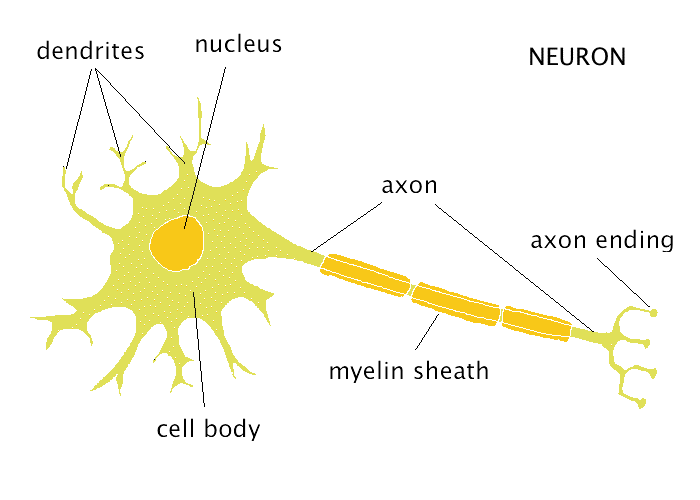
\includegraphics[width=\imgwidth]{bio_neuron}
  \caption{A schematic of biological neuron}
  \label{fig:bioneuron}
\end{figure}

\paragraph{Artificial neurons} 

In fact, artificial neuron can be viewed as a parametric function of $ n $ inputs $ g_{w}:X^{n} \rightarrow Y $, where X is the space of all possible input values, Y - the space of output values and w - the vector of numeric weights $ w_{1}, w_{2}, ..., w_{n} $, the tunable parameters that [...]. In other words, function $ g_{w} $ is [defined with the rule]

\begin{equation}
  y = g_{w}(x)
\end{equation}

where $ x \in X^{n} $, $ y \in Y $ and $ w \in \mathbb{R}^{n} $.

Function $ g_{w} $ is a superposition of two functions, $ s_{w}:X^{n} \rightarrow \mathbb{R} $ and $ f:\mathbb{R} \rightarrow Y $:
\[ g_{w}(x) = f(s_{w}(x)) \]

where $ s_{w} $ is defined as follows:
\[ s_{w}(x) = \sum_{i=0}^{n} w_{i}x_{i} \]

$ f $ is a nonlinear activation function in case of classification and an identity function $ \forall x f(x) = x $ in case of regression.

\begin{figure}[H]
  \centering
  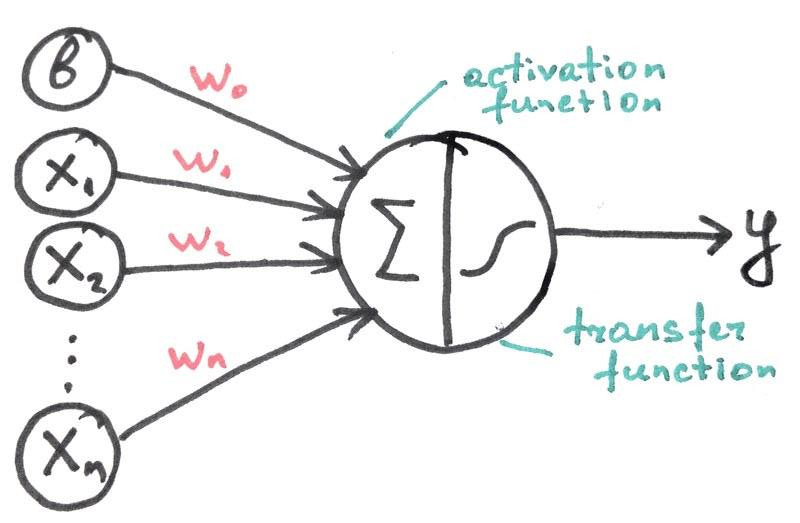
\includegraphics[width=0.8\imgwidth]{artif_neuron}
  \caption[Model of an artifitial neuron]{Model of an artifitial neuron\footnotemark}
  \label{fig:artifneuron}
\end{figure}

\footnotetext{Source: \url{http://www.theprojectspot.com/tutorial-post/introduction-to-artificial-neural-networks-part-1/7}}

%[By type of activation function neurons are divided ...
%Hard and soft thresholds
%
%Neurons with  hard thresholds are called \textbf{perceptrons}.


\section{Structure and representation}
\paragraph{Graphical representation} Neural networks are composed of nodes (neurons), connected by direct links (synaptic connections). If we think of neurons as vertices and synaptic connections as edges, neural networks can be represented by weighted directed graphs called \textbf{network diagrams}.

If the network is feedforward (without cycles), the graph will be $ k $-partide, where $ k $ is the number of layers. If it is also fully-connected, it will be a complete $ k $-partide graph. See Figure \ref{fig:graphs} for specific examples.

\begin{figure}[H]
  \centering
  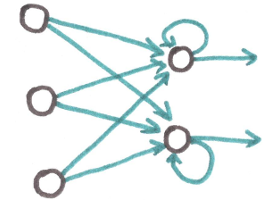
\includegraphics[width=0.3\textwidth]{recurrent}
  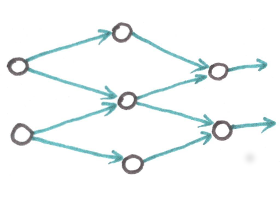
\includegraphics[width=0.3\textwidth]{feedfwd}
  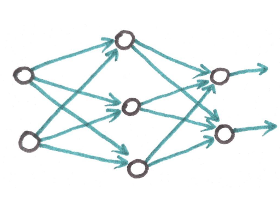
\includegraphics[width=0.3\textwidth]{full_feedfwd}
  %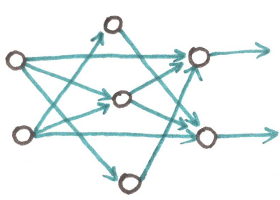
\includegraphics[width=0.4\textwidth]{nonpart_feedfwd}
  \caption{(1) Recurrent neural network represented by directed graph. (2) 3-layered feedforward neural network represented by 3-partide directed graph. (3) 3-layered fully-connected feedforward neural network represented by a complete 3-partide directed graph}
  \label{fig:graphs}
\end{figure}

\paragraph{Network topologies}
As it was already said, neural networks consist of neurons. These neurons are connected with directed links (synaptic connections) with numeric weights that determine the strength and sign of the connection.

Neurons are grouped into layers. First layer is called \textbf{input layer}, the last one - \textbf{output layer}. All the layers between input and output layers are called \textbf{hidden layers}. Number of hidden layers is one of the tunable metaparameters that define the architecture of a neural network. According to \cite{Hastie-et-al-2013}, typically the number of hidden units is somewhere in the range of 5-100.

To satisfy the linear model of a regression each layer, except for the output one, has an additional bias unit $ b = 1 $.

For a specific example of neural network architecture see Figure \ref{fig:net}.

By the type of connections neural network can be either feedforward or recurrent:
\begin{itemize}
  \item \textbf{Feedforward network} - has connections only in one direction (outputs of neurons from layer $ k $ can be connected only to neurons of layers $ k + c $ where $ c > 0 $). The network diagram of a feedforward netwond forms a directed acyclic graph.
  \item \textbf{Recurrent network} - feeds its outputs to its own inputs. This network has at least one cycle (at least one connection from neuron in layer $ k $ to neuron in layer $ k - c $ where $ c \geq 0 $). 
\end{itemize}
  
If in neural network with $ N $ layers $ \forall k:0 \leq k \leq N-1  $ every neuron in layer $ k $ is connected to all the neurons of layer $ k+1 $, the network is called \textbf{fully-connected}.
  
Figure \ref{fig:net} depicts the schematic of a feedforward neural network with one hidden layer.
  
\begin{figure}[H]
  \centering
  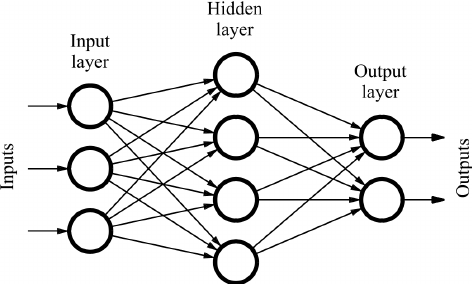
\includegraphics[width=\imgwidth]{net}
  \caption[Feedforward artificial neural network]{Feedforward artificial neural network with one hidden layer. Number of neurons in each layer: 3 (2-dimentional input + bias unit) in the input layer, 4 in the hidden layer, 1 in the output layer (1-demensional output)\footnotemark}
  \label{fig:net}
\end{figure}

\footnotetext{Source: \url{https://www.researchgate.net/figure/234055177_fig1_Figure-61-Sample-of-a-feed-forward-neural-network}}


\section{Training a neural network}
In this section I will describe gradient descent and the backpropagation learning algorithm. One of the most important features of backpropagation, which makes it so popular is that it can be easily parallelized.

\subsection{Gradient descent}
The most widely used algorithm for training neural networks (and optimizing many other machine learning problems) is called gradient descent. It is based on the fact that derivative (gradient) of a function characterizes how how it grows:
\begin{itemize}
  \item The sign of a derivative over some parameter denotes the direction in which the function grows
  \item The ablsolute value of derivative tells us how fast the function grows
\end{itemize}
Therefore, derivative of a function at some point can tell us in which direction and how far should we move to minimize the function.

This helps us construct an algorithm for function minimization which is based on adding some gradient to the value of parameter.

Let's say we have a cost function $J(t;w)$ that depends on the target output $t$ that we expect our model to produce, and the tunable parameter $w$ (weight). To minimize this function we change the weight $w$ by the value of gradient $-\eta\frac{\partial}{\partial w}J(t;w)$ until the function reaches the minimum (gradient becomes equal to 0.

\begin{equation}
  w = w - \eta\frac{\partial}{\partial w}J(t;w) 
\end{equation}

The parameter $\eta$ is called the learning rate. It controlls the speed of learning. If $\eta$ is big, we are making big steps in the directions in which our function descends. This means that the model learns faster, but also creates the risk of overshooting - we can jump too far to the point where the function increases again. This may result in divergence - the situation when our model keeps getting worse instead of getting better. Another problem arises when the $\eta$ is too small. First of all, such learning algorithm could take unreasonable amount of time to converge. And if the cost function that we are trying to minimize is nonlinear, we may get stuck in a local minimum. Choosing a good leraning rate is one of the hardest tasks of machine learning.

\subsection{Backpropagation}
As the number of hidden layers grows, the problem arises, as we can only compute the error of output layer by finding the deviation of hypothesis $ h_{w} $ from the desired output $ y $.

The fitness function for regression is the sum of squared errors
 
\begin{equation}
  J(w) = \sum_{k=1}^{K} \sum_{i=1}^{n} (y_{i} - f_{k}(x_{i}))^{2}
\end{equation}

For classification it is defined as

\begin{equation}
  J(w) = \sum_{i=1}^{n} y_{ik} \log{f_{k}(x_{i}}
\end{equation}

The task of learning is to minimize the fitness function $ J(w) $. There are different learning algorithms for doing that. In this paper I will explain only the idea of the classical backpropagation algorithm.

Backpropagation is an abbreviation for "backward propagation of errors". According to \cite{Hastie-et-al-2013}, backpropagation is a two-pass procedure, used to compute the gradients for the updates in gradient descent algorithm:

\begin{itemize}
  \item \textbf{Forward pass} -the current weights are fixed and the predicted values are computed
  \item \textbf{Backward pass} - the errors $ \delta_{ki} $ are computed and then backpropagated to give errors $ s_{ij} $. Both sets of errors are then used to compute the gradients for updates.
\end{itemize}

The main advantage of backpropagation is that it has local nature, and thus it can be efficiently implemented on a parallel architecture computer.

%\begin{align}
%J(w) = &-\frac{1}{m} \bigg[ \sum_{i=1}^{m} \sum_{k=1}^{K}
%    y_{k}^{(i)} \log{(h_{w}(x^{(i)}))_{k}}
%    + (1 - y^{(i)}) \log{1 - (h_{w}(x^{(i)}))_{k}}) \bigg] \\
%    % Regularization
%    &+ \frac{\lambda}{2m}
%    \sum_{l=1}^{L-1} \sum_{i=1}^{S_{l}} \sum_{j=1}^{S_{l+1}}
%    (W_{ji}^{(l)})^{2}
%\end{align}

%[Backpropagation is usually considered to be a supervised learning method, although it is also used in some unsupervised networks - from Wikipedia, needs verification]

